\documentclass[11pt, letterpaper]{article}

% ---------- packages ----------
\usepackage[margin=0.7in]{geometry}
\usepackage{tcolorbox}
\usepackage{enumitem}
\usepackage{hyperref}
\usepackage{xcolor}
\usepackage{titlesec}
\usepackage{fancyhdr}
\usepackage{graphicx}
\usepackage{tabularx}
\usepackage{booktabs}

% ---------- colors ----------
\definecolor{boxborder}{RGB}{60, 90, 150}
\definecolor{boxbg}{RGB}{245, 248, 255}
\definecolor{headcolor}{HTML}{00636f}
\definecolor{placeholder}{RGB}{140, 140, 140}

% ---------- tcolorbox style ----------
\tcbset{
  sectionbox/.style={
    colframe=boxborder,
    colback=boxbg,
    boxrule=0.6pt,
    arc=2pt,
    left=6pt, right=6pt, top=4pt, bottom=4pt,
    fontupper=\small,
  }
}

% ---------- placeholder command ----------
\newcommand{\placeholder}[1]{\textcolor{placeholder}{\textit{#1}}}

% ---------- section formatting ----------
\titleformat{\section}
  {\normalsize\bfseries\color{headcolor}}{\thesection.}{0.4em}{}
\titlespacing*{\section}{0pt}{6pt}{2pt}

% ---------- header / footer ----------
\pagestyle{fancy}
\fancyhf{}
\renewcommand{\headrulewidth}{0.4pt}
\lhead{\small\color{headcolor} CS 4100 -- Project Executive Summary}
%\rhead{\small\color{headcolor} Semester, Year}
\cfoot{\small\thepage}

% ---------- suppress paragraph indent ----------
\setlength{\parindent}{0pt}
\setlength{\parskip}{3pt}

\begin{document}

% ===== TITLE BLOCK =====
\begin{center}
  {\Large\bfseries\color{headcolor} Movie Recommendation System}\\[4pt]
  {\normalsize Alexander Park, Shariq Rifai, Haozhe Shi}\\[2pt]
\end{center}

\vspace{4pt}

% ===== 1. MOTIVATION & PROBLEM STATEMENT =====
\section{Motivation \& Problem Statement}
\begin{tcolorbox}[sectionbox, height=4.6cm, valign=top]
  % --> REMOVE THE \placeholder ENV BELOW, AND ADD YOUR OWN TEXT  <-- %
  \placeholder{%
    Describe the real-world problem your project addresses and explain
    why it matters. Identify the specific gap, limitation, or
    opportunity that motivates this work. State the core research
    question or engineering goal in one clear sentence.
    Cite relevant prior work or context that frames the problem
    (1--2 references are sufficient). Aim for roughly 8--12 sentences.}
    
    With so many movies out there and the length of a movie being such a large time commitment, it is difficult to find a new movie that you might like. It can also a struggle to find a movie that has the same ‘vibe’ as another movie, and a viewer might not know what draws them to that specific ‘vibe.’ Streaming services already recommend shows and movies based on user preferences, such as the "Recommended" section on Netflix, but people remain unsatisfied with those recommendations and stay unsure of what to watch next. A good movie recommendation model with customizable inputs can solve this problem.
\end{tcolorbox}

% ===== 2. APPROACH =====
\section{Approach}
\begin{tcolorbox}[sectionbox, height=7.0cm, valign=top]
% --> REMOVE THE \placeholder ENV BELOW, AND ADD YOUR OWN TEXT  <-- %
  \placeholder{%
    Summarize your technical approach at a high level. Describe the
    system architecture or methodology, key algorithms or models used,
    and the most important design decisions. If applicable, include a
    small figure or diagram (use \textbackslash includegraphics), and resize to stay within bounded box area.
    Mention the primary tools, frameworks, or libraries
    (e.g., PyTorch, Mesa, Gymnasium, PettingZoo).
    Clearly state any assumptions or scope limitations.
    Aim for roughly 10--15 sentences or equivalent with an optional figure.}

    Our model takes in a list of movies that the user has already watched in the past and enjoyed. The user can then optionally enter a genre constraint to only include movies from that genre in the output. From there, the model recommends a movie to the user, and the user can say yes or no. If the user says no, the model will try again and recommend a different movie. The user can repeat as many times as desired.

    The recommendation model itself has 2 stages: heuristic scoring and a neural network. The heuristic scoring stage compares attributes from the movies that the user enjoys with potential movie recommendations. Some heuristics that are scored are actors, genre, IMDB rating, and keywords. The keywords are generated from an LLM which is prompted to generate 10 keywords to describe a movie's plot, and the other heuristics are retrieved from the Open Movie Database API. 
\end{tcolorbox}

% ===== 3. KEY RESULTS =====
\section{Key Results}
\begin{tcolorbox}[sectionbox, height=8cm, valign=top]
% --> REMOVE THE \placeholder ENV BELOW, AND ADD YOUR OWN TEXT  <-- %
  \placeholder{%
    Present the most important quantitative and/or qualitative results.
    Include 1--2 key metrics, comparisons, or summary statistics.
    Interpret the results: what worked well, what was surprising,
    and how do the outcomes compare with your initial expectations
    or baselines? Aim for roughly 8--12 sentences or equivalent. Small tables, figures, or charts may be embedded here, and/or in the first box on the next page (examples on next page).}
    
\end{tcolorbox}

\newpage

\begin{tcolorbox}[sectionbox, height=8cm, valign=top]
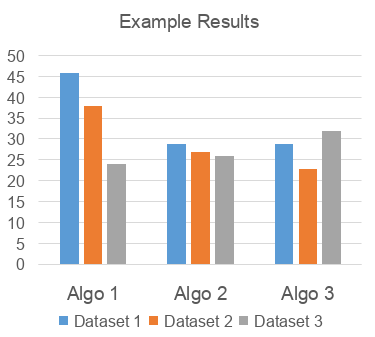
\includegraphics[width=0.42\linewidth]{Picture.png}\hfill
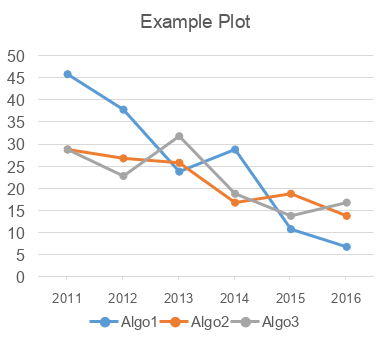
\includegraphics[width=0.42\linewidth]{Picture2.png}
  \\
  % --> REMOVE THE \placeholder ENV BELOW, AND ADD YOUR OWN TEXT  <-- %
  \placeholder{%
  Replace these figures with your own, or remove them and use this space for more text. Ensure all text in your figures are clear and readable at this scale, similar to these examples.
   }
\end{tcolorbox}
% ===== 4. CHALLENGES & LESSONS LEARNED =====
\section{Challenges \& Lessons Learned}
\begin{tcolorbox}[sectionbox, height=4.4cm, valign=top]
% --> REMOVE THE \placeholder ENV BELOW, AND ADD YOUR OWN TEXT  <-- %
  \placeholder{%
    Discuss the main technical and organizational challenges
    encountered during the project. For each challenge, briefly
    explain how the team addressed or mitigated it.
    Highlight lessons learned that would be valuable for future
    work or for other teams tackling similar problems.
    Aim for roughly 8--12 sentences.}
    
    We definitely faced some challenges with communication since we all have our own schedules and were always busy with other work. There were some meetings we held in which one of us was unable to meet and had to be filled in afterwards. We addressed this by staying active in the group chat to communicate when we do/don't have time at certain points, and staying organized with a design document and repository. With this, even if we weren't all able to meet, we could catch up by reading updates on these platforms and keeping an open line of communication if any questions arise. 
\end{tcolorbox}

% ===== 5. INDIVIDUAL CONTRIBUTIONS =====
\section{Individual Contributions}
\begin{tcolorbox}[sectionbox, height=4.3cm, valign=top]
  \vspace{4pt}
  \centering
  \begin{tabularx}{0.95\textwidth}{l X c}
    \toprule
    \textbf{Member} & \textbf{Primary Contributions} & \textbf{Approx.\ \%} \\
    \midrule
    Alex & System and environment design, project management, dataset & 33\% \\
    Shariq & LLM setup, CLI user interface & 33\% \\
    Haozhe & API setup, Neural network model implementation & 33\% \\
    \bottomrule
  \end{tabularx}
\end{tcolorbox}

% ===== 6. REPOSITORY & REFERENCES =====
\section{Repository \& References}
\begin{tcolorbox}[sectionbox, height=4.5cm, valign=top]
  \textbf{GitHub Repository:}
       {\texttt{https://github.com/alexpark0/CS4100-Group-Project}}\\
\vspace{1pt}

  \textbf{Project Tracker:} {\texttt{https://github.com/users/alexpark0/projects/1/views/1}}

  \vspace{6pt}
  \textbf{Key References:}
  \begin{enumerate}[leftmargin=1.4em, itemsep=1pt, topsep=2pt, label={[\arabic*]}]
    \item \placeholder{Author(s), ``Title,'' Venue, Year. Brief annotation.}
    \item \placeholder{Author(s), ``Title,'' Venue, Year. Brief annotation.}
    \item \placeholder{Author(s), ``Title,'' Venue, Year. Brief annotation.}
  \end{enumerate}

  \vspace{4pt}
  \placeholder{Add or remove reference entries as needed (3--4 recommended).}
\end{tcolorbox}

\end{document}